\documentclass[10pt,a4paper]{article}
\usepackage[utf8x]{inputenc}
\usepackage{ucs}
\usepackage[english]{babel}
\usepackage{amsmath}
\usepackage{amsfonts}
\usepackage{amssymb}
\usepackage{makeidx}
\usepackage{graphicx}
\usepackage{lmodern}
\usepackage{kpfonts}
\usepackage{float}

\usepackage[left=2cm,right=2cm,top=2cm,bottom=2cm]{geometry}

\usepackage{titlesec}


% elimina newline despues de \section:
\titleformat{\section}[runin]
{\normalfont\large\bfseries}{\thesubsection}{1em}{}


\headsep17mm
\topmargin-1cm
\hoffset -1.5cm \voffset -1cm \textwidth 17cm \oddsidemargin
1.5cm \evensidemargin 1.5cm \textheight 22.5cm

\begin{document}

\vspace{0,3cm}

\begin{center}
{\bf \Large Resoluciones seleccionadas, semana 01}
\end{center}

\vspace{0,3cm}

\section*{2.1.j}\emph{Calcular las raices de $P(x) = x^4-x^2-2$}


\noindent
\emph{Solución:}


\noindent
Los polinomios de esta forma (grado 4 con coeficientes en la primer y tercer
potencia nulos) pueden transformarse y resolverse como si fuesen de segundo
grado.
Consideramos el cambio de variable
$u := x^2$. El polinomio queda $P(x) = Q(u) = u^2-u-2$,
cuyas raices (en función de $u$), aplicando la f\'ormula
de Bhaskara son:

\begin{equation*}
  \begin{split}
    &u_1 = \frac{1 + \sqrt{(-1)^2-4\cdot 1 \cdot (-2)}}{2 \cdot 1} = 2\\
    &u_2 = \frac{1 - \sqrt{(-1)^2-4\cdot 1 \cdot (-2)}}{2 \cdot 1} = -1
  \end{split}
\end{equation*}

\noindent
Luego, encontramos los $x$ para los cuales $u$ toma esos valores.
Es decir, resolvemos las ecuaciones $x^2 = u_i$
para obtener las raices de $P(x)$.
De $x^2=2$ obtenemos $x_1=\sqrt{2}$, $x_2 = \sqrt{2}$. De $x^2=-1$ no se obtienen nuevas
raices reales. Si estamos trabajando en el cuerpo de los complejos,
obtenemos
$x_3 = i$, y $x_4 = -i$.

\noindent
Notar que este procedemiento se puede emular si los exponentes tienen un divisor común, por ejemplo para el polinomio $x^{10} - x^{5} - 2$.

\section*{3.2.j}
\emph{Determinar para qué valores de $x$ es cierta la siguiente inecuaci\'on:}

\begin{equation*}
  \vert 2x - 5 \vert  <  \vert 3x + 4 \vert
\end{equation*}



\noindent
\emph{Solución:}

\noindent
Recordemos la definición de valor absoluto:
\begin{equation*}
  \vert x \vert =
  \begin{cases}
    x & \mbox{si } x\geq 0 \\
   -x & \mbox{si } x < 0
  \end{cases}
\end{equation*}

\noindent
Observemos que esta función está definida por tramos
\footnote{https://en.wikipedia.org/wiki/Piecewise},
la expresión algebraica depende del signo de $x$.
Para decidir cuanto vale $|2x - 5|$, estudiamos el signo de $2x-5$.
Si $2x-5 \geq 0$ entonces $|2x-5| = 2x-5$. De lo contrario $|2x-5| = -2x+5$,
el opuesto. Análogamente, razonamos para $ 3x+4$.

\begin{center}
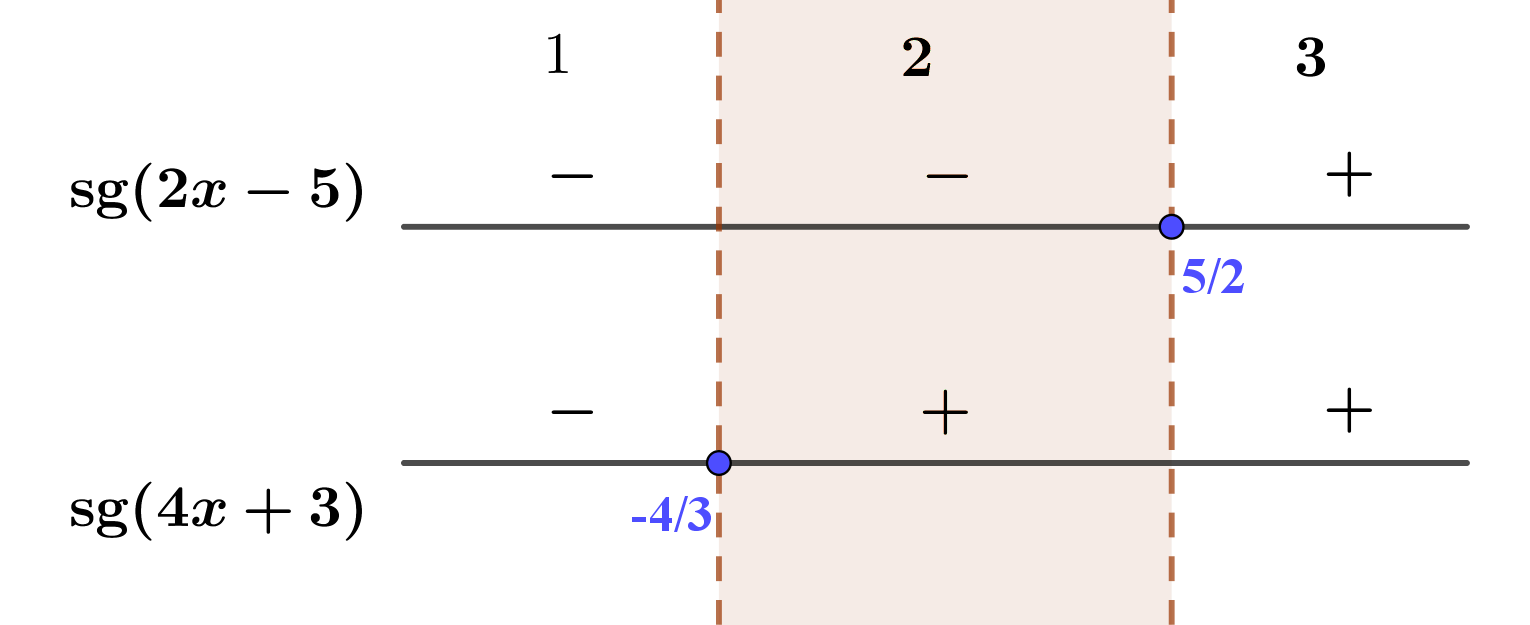
\includegraphics[width=100mm]{signo}
\end{center}

\newpage

El dominio nos queda dividido entonces en tres regiones:
\begin{enumerate}
\item
  Si $x \in \left(-\infty, \frac{-4}{3}\right)$ tenemos que $|2x-5| = -2x+5$ y que
  $|3x+4| = -3x-4$.
  La ecuación a estudiar en este intervalo es $ -2x+5 < -3x-4$.
  Reduciendo:
  \begin{align*}
    -2x+5 <& -3x-4    & \iff \\
    5 + 4 <& -3x + 2x & \iff \\
    9     <& -x       & \iff \\
    x     <& -9 &
  \end{align*}

  La solución obtenida {\bf solo tiene sentido en la región estudiada},
  por tanto para la solución final nos interesa el conjunto
  $$(-\infty, -9) \cap \left(-\infty, \frac{-4}{3}\right) = (-\infty, -9)$$
  (La solución obtenida, intersección la región estudiada, en este caso da
  lo mismo).
  
\item
  Si $x \in \left[\frac{-4}{3}, \frac{5}{2}\right)$ tenemos que $|2x-5| = -2x+5$ y que
  $|3x+4| = 3x+4$.
  La ecuación a estudiar en este intervalo es $ -2x+5 < 3x+4$.
  Reduciendo:
  \begin{align*}
    -2x+5  <& 3x+4     & \iff \\
     5 - 4 <& 3x + 2 x & \iff \\
     1     <& 5x       & \iff \\
     x     >& \frac{1}{5} &\\
  \end{align*}

  Por tanto {\bf en la región} la solución es
  $\left\lbrace x\in \mathbb{R} : x > \frac{1}{5}\right\rbrace$, y aporta a la solución total
  el conjunto \newline
  
  $$\left\lbrace x\in \mathbb{R} : x > \frac{1}{5}\right\rbrace \cap \left[\frac{-4}{3}, \frac{5}{2}\right)   = \left(\frac{1}{5}, \frac{5}{2}\right)$$

  (Una vez más es la solución obtenida, intersección la región estudiada,
  en este caso queda clara la diferencia).
  

\item
  Si $x \in \left[\frac{5}{2},\infty\right)$ tenemos que $|2x-5| = 2x-5$ y que
  $|3x+4| = 3x+4$.
  La ecuación a estudiar en este intervalo es $ 2x-5 < 3x+4$.
  Reduciendo:
  \begin{align*}
    2x-5  <& 3x+4       & \iff \\
     -5 - 4 <& 3x - 2 x & \iff \\
     x >& -9 \\
  \end{align*}

  \noindent
  Por tanto en la región la solución es
  $\{ x\in \mathbb{R} : x > -9 \}$, y aporta a la solución total al conjunto
  $\{ x\in \mathbb{R} : x > -9 \} \cap [\frac{5}{2},+\infty)
    = [\frac{5}{2},+\infty)$
  
\end{enumerate}

Finalmente, el conjunto solución está dado por la unión de las soluciones
de cada intervalo, y es el conjunto:

$$(-\infty, -9) \cup \left(\frac{1}{5}, \frac{5}{2}\right) \cup \left[\frac{5}{2},+\infty\right)
  = (-\infty, -9) \cup \left(\frac{1}{5}, +\infty\right)$$




\end{document}
